\begin{document}
\maketitle

\begin{abstract}
A minimal carrier $E_3\oplus E_2$ on the oriented double cover is shown to be the unique rank-5 split satisfying $\dim\Lambda^{\mathrm{even}}E=16$ and $\tr_EY^2=5/6$. This carrier already forces the global Standard Model group $S(U(3)\times U(2))\cong(SU(3)\times SU(2)\times U(1)_Y)/\mathbb Z_6$, one chiral family with $\nu^c$ from the positive half-spinor, the hypercharge--seam inversion $6Y^2-Y-\mathbf 1=0$, and a self-consistent electromagnetic closure equation whose retained canonical branch is later compared to $\alpha^{-1}(0)=\num{137.0359992}$.

Under the declared admissibility, $\APSdom/\APSfam$, Bernstein-kernel positivity, and reflection-positivity axioms, the same carrier-first architecture closes into an operative selector $\Padm$, an APS family theorem with $\Ind_{APS}(D^+_{\mathrm{rel}}\otimes L_F)=3$, a bosonic relative index selecting one seam-even Higgs doublet, a local-spectral-scale closure for $\Mpl$ and $\vgeo$, a holonomy form of the Yukawa matrices, a hadronic Hilbert space $\Hhad=\overline{\Asing|\Omega\rangle}$, anomaly cancellation with seam inflow, a Lorentzian reconstruction from relative reflection positivity, and an admissible vacuum minimizer with renormalized seam vacuum energy $\Lambda_{\Seam,\mathrm{ren}}$.

Compression identities and benchmark discipline remain visible rather than decorative: the rank-lock $2^{g-3}=g-1$ fixes $g=5$, the hard $41$-chain $10\,b_1=\Omega_{\mathrm{adm}}\gamma+1=41$ overdetermines the canonical branch, the Cabibbo inversion $\phiz=\frac12(1-\sqrt{1-4\lambda_C^2})$ compresses the bridge observables into one retained seed, and wrong discrete worlds still fail the electromagnetic closure decisively. The comparison map $\mathcal R_{\SM}$ is kept explicit at $\mu_{\mathrm{match}}=M_Z$ with the declared threshold set $\{m_c,m_b,m_\tau,m_t\}$, while E$_8$ scale grammar and horizon language remain the main conditional appendix layers.
\end{abstract}

\begin{tcolorbox}[colback=gray!5, colframe=gray!60, breakable,
    title={\textbf{Reading Status for the Present Paper}}, fonttitle=\bfseries]
\begin{itemize}[leftmargin=1.5em, topsep=3pt, itemsep=3pt]
    \item \textbf{Primitive datum:} oriented double cover, seam $\Seam$, involution $\inv$, the relative Dirac pair, the internal finite Hilbert space $\Hint$, the Bernstein spectral test function $f$, and the primitive seam response $\chiseed$.
    \item \textbf{Hard carrier/kernel:} minimal carrier $E_3\oplus E_2$, global group $S(U(3)\times U(2))\cong \frac{SU(3)\times SU(2)\times U(1)_Y}{\mathbb Z_6}$, one chiral family, carrier norm $5/6$, the abelian-index formula $\bone(N_{\mathrm{fam}},N_\Phi)$, seam normalization $\cthree$, base opening $\phibase$, and the carrier-form electromagnetic closure equation.
    \item \textbf{Closed from the admissibility complex:} the operative selector $\Padm$, the imported APS family theorem and $\Oadm=48$, Callias Higgs selection, the local spectral-scale / gravity closure for $\Mpl$ and $\vgeo$, Yukawa holonomy, hadronic space, anomaly/inflow cancellation, strong CP, nonperturbative QFT closure, reflection positivity, Lorentz reconstruction, stable record algebra, main-text prediction semantics, and admissible vacuum closure with $\Lambda_{\Seam,\mathrm{ren}}$.
    \item \textbf{Benchmark bridge:} the comparison map $\mathcal R_{\SM}$, the retained transport saddle $\delta_{\mathrm{ph}}$, the canonical numeric value $\bone=41/10$, the evaluated benchmark rows such as $\alpha^{-1}(0)$, the declared thresholds, and the ledger interface from compiler outputs to scheme-specified observables.
    \item \textbf{Conditional extensions:} downstream E$_8$ scale grammar, horizon language, and appendix-level long-range extrapolations.
\end{itemize}
\end{tcolorbox}

\tableofcontents

\section{Reading guide and claim map}

The paper is organized in three reading layers:
\begin{itemize}[leftmargin=1.5em, topsep=3pt, itemsep=2pt]
    \item \textbf{Big picture:} one section explains what TFPT claims in plain language before the detailed datum and conventions begin.
    \item \textbf{Detail:} the main body then runs from primitive core and hard carrier kernel through kernel numerics, the two closure-architecture sections, the closure theorem stack, the particle/mass compiler, and the benchmark interface.
    \item \textbf{Proof sketches:} the main text gives only the central proof sketches, while dense technical derivations remain in appendices or companion material.
\end{itemize}
The status language is also fixed once and for all:
\begin{itemize}[leftmargin=1.5em, topsep=3pt, itemsep=2pt]
    \item \textbf{Primitive datum} means the undecomposed relative spectral starting package used before any carrier, family, or admissibility closure is derived.
    \item \textbf{Hard} means established carrier or kernel structure that does not use the later closure axioms.
    \item \textbf{Closed from the admissibility complex} means theorem-level closure once the admissibility differential, the imported family theorem, and the declared $\APSfam$ / Bernstein / reflection-positivity inputs are imposed.
    \item \textbf{Benchmark bridge} means the declared map from compiler outputs to scheme-specified observables.
    \item \textbf{Conditional extension} means a downstream or appendix-level statement not needed for the present closed compiler surface.
\end{itemize}
To keep theorem language, benchmark semantics, and appendix bookkeeping lexically stable, all prose, captions, and status labels are kept in English throughout.

\begin{tcolorbox}[colback=gray!4, colframe=gray!60, breakable,
    title={\textbf{Datum Hierarchy for the Present Draft}}, fonttitle=\bfseries]
\begin{itemize}[leftmargin=1.5em, topsep=3pt, itemsep=3pt]
    \item \textbf{Primitive datum:} oriented double cover, seam $\Seam$, involution $\inv$, the finite internal space $\Hint$, the relative operator framework, the Bernstein spectral kernel, and the primitive seam response $\chiseed$.
    \item \textbf{Derived hard kernel:} minimal carrier $E_3\oplus E_2$, the internal quotient $S(U(3)\times U(2))$, one-family packet $S^+$, hypercharge--seam inversion, the coefficient function $\bone(N_{\mathrm{fam}},N_\Phi)$, seam normalization $\cthree$, base opening $\phibase$, and the electromagnetic closure equation.
    \item \textbf{Closure layer:} $\Padm$, the imported APS family theorem, Callias Higgs selection, local spectral-scale / gravity closure, transport-side mass closure, strong CP, nonperturbative QFT closure, anomaly inflow, Lorentz/OS reconstruction, stable record algebra, prediction semantics, and vacuum existence with $\Lambda_{\Seam,\mathrm{ren}}$.
    \item \textbf{Benchmark layer:} the comparison map $\mathcal R_{\SM}$, the retained transport saddle $\delta_{\mathrm{ph}}$, the evaluated canonical value $\bone=41/10$, threshold discipline, and benchmark ledgers.
\end{itemize}
\end{tcolorbox}

\begin{figure}[t]
\centering
\begin{tikzpicture}[
    scale=0.58,
    transform shape,
    >=Latex,
    node distance=1.6cm and 1.7cm,
    primitive/.style={draw=gray!70!black, thick, rounded corners, fill=gray!10, align=center, minimum width=2.8cm, minimum height=1cm},
    hard/.style={draw=blue!60!black, thick, rounded corners, fill=blue!4, align=center, minimum width=2.8cm, minimum height=1cm},
    bridge/.style={draw=green!50!black, dashed, thick, rounded corners, fill=green!4, align=center, minimum width=2.9cm, minimum height=1cm},
    closure/.style={draw=orange!70!black, dotted, thick, rounded corners, fill=orange!5, align=center, minimum width=3.0cm, minimum height=1cm},
    conditional/.style={draw=purple!70!black, dash pattern=on 4pt off 2pt on 1pt off 2pt, thick, rounded corners, fill=purple!5, align=center, minimum width=3.0cm, minimum height=1cm}
]
\node[primitive] (core) {$\Tprim$\\primitive datum and spectral seed};
\node[hard, right=of core] (carrier) {$\Tker$\\carrier packet and one family};
\node[closure, right=of carrier] (bridge) {$\Padm$, $F$, $\Oadm$\\closure selector and family theorem};
\node[closure, below=of carrier] (geom) {$\Ageom$\\Higgs, $\sigma/\chigeo$, superconnection};
\node[closure, below=of bridge] (trans) {$\Atrans$\\Yukawas, confinement, strong CP};
\node[bridge, right=of bridge] (cmp) {compiler interface\\RG map, ledgers, benchmarks};
\node[conditional, below=of cmp] (cond) {conditional layer\\E$_8$ and horizons};
\draw[->, thick] (core) -- (carrier);
\draw[->, thick] (carrier) -- (bridge);
\draw[->, dotted, thick] (carrier) -- (geom);
\draw[->, dotted, thick] (bridge) -- (trans);
\draw[->, dashed, thick] (bridge) -- (cmp);
\draw[->, dotted, thick] (geom) -- (cmp);
\draw[->, dotted, thick] (trans) -- (cmp);
\draw[->, dash pattern=on 4pt off 2pt on 1pt off 2pt, thick] (cmp) -- (cond);
\coordinate (legone) at ($(geom.south west)+(-0.9,-2.3)$);
\draw[->, thick, gray!70!black] (legone) -- ++(1.2,0) node[right, black, font=\scriptsize] {Primitive datum};
\coordinate (legtwo) at ($(legone)+(0,-0.6)$);
\draw[->, thick] (legtwo) -- ++(1.2,0) node[right, black, font=\scriptsize] {Hard};
\coordinate (legthree) at ($(legtwo)+(0,-0.6)$);
\draw[->, dotted, thick] (legthree) -- ++(1.2,0) node[right, black, font=\scriptsize] {Closure};
\coordinate (legfour) at ($(legthree)+(0,-0.6)$);
\draw[->, dashed, thick] (legfour) -- ++(1.2,0) node[right, black, font=\scriptsize] {Benchmark bridge};
\coordinate (legfive) at ($(legfour)+(0,-0.6)$);
\draw[->, dash pattern=on 4pt off 2pt on 1pt off 2pt, thick, purple!70!black] (legfive) -- ++(1.2,0) node[right, black, font=\scriptsize] {Conditional extension};
\end{tikzpicture}
\caption{Claim map for the carrier-first compiler form across primitive datum, hard kernel, closure layer, benchmark bridge, and conditional extensions.}
\label{fig:dependency-map}
\end{figure}

\begin{table}[t]
\centering
\scriptsize
\begin{tabularx}{\linewidth}{@{}>{\raggedright\arraybackslash}p{0.23\linewidth}>{\raggedright\arraybackslash}p{0.12\linewidth}YY@{}}
\toprule
Layer or statement & Status & Proof source or missing lemma & Main empirical or structural test \\
\midrule
Primitive relative spectral datum and Bernstein spectral action & Primitive datum & primitive spectral package and well-posedness theorem in the main text & failure would collapse the operator-level starting point \\
Oriented double cover, seam, involution & Hard & starting geometric datum; fixed throughout the paper & structural consistency of all later layers \\
Minimal carrier $E_3\oplus E_2$ & Hard & proof sketch given in \Cref{sec:minimal-carrier-proof} & failure would collapse the whole packet \\
One-family packet $S^+=\Lambda^{\mathrm{even}}E$ & Hard & decomposition and proof sketch given in the main text & group/matter mismatch would be global \\
Carrier coefficient function $\bone(N_{\mathrm{fam}},N_\Phi)$ & Hard & abelian-index formula in the main text & hypercharge-trace mismatch would be structural \\
Hard seam/kernel constants $(\cthree,\phibase,\deltatop)$ & Hard & seam normalization, base opening, and carrier-form closure equations summarized in the main text & scheme discipline for observable comparison \\
Canonical closure value $\bone=41/10$ & Closure & canonical family/Higgs closure of the abelian index on the retained branch & failure would break the 41-chain and the canonical packet count \\
Operative admissibility selector $\Padm$ & Closure & closure theorem stack in \Cref{sec:closure-theorems} & unified electroweak / QCD / CP sector selection \\
Family APS theorem, $F\cong\mathbb C^3$, and $\Oadm=48$ & Closure & imported orbifold--APS family theorem plus occupancy corollary in \Cref{sec:closure-theorems}; full derivation remains a named proof obligation & flavor multiplicity and family lifting \\
Bosonic relative index selecting $\Phi$ & Closure & Callias Higgs-selection theorem and bosonic closure theorem in \Cref{sec:closure-theorems} & unique light doublet / doublet-triplet split \\
Local spectral-scale / gravity closure for $\Mpl$ and $\vgeo$ & Closure & bosonic closure theorem, gravity/cosmology theorem, and two-sheet zero-mode lemma & Planck / electroweak / gravity relation \\
Yukawa holonomy matrix and mass closure & Closure / retained rule & transport holonomy grammar plus retained admissible packets, gap lift, and holonomy-triangle phase control & $m_f$, CKM / PMNS, hierarchy grammar \\
Hadronic space, anomaly inflow, and strong CP & Closure & hadronic / anomaly closure theorems in \Cref{sec:closure-theorems} & hadron spectrum and $\bar\theta$ null tests \\
Nonperturbative QFT closure & Closure & gap lift, Callias positivity bounds, and admissible QFT theorem & mass gap, clustering, and confinement route \\
Reflection positivity, Lorentz reconstruction, record algebra, and vacuum closure & Closure & relative generating functional, admissible reflection-positivity lemma, gap/clustering record construction, split OS / vacuum theorems, and primitive Lorentzian corollary & causal dynamics, stable records, and vacuum energy map \\
Comparison map $\mathcal R_{\SM}$, $\alpha^{-1}(0)$, and transport saddle $\delta_{\mathrm{ph}}$ & Benchmark bridge & declared RG / threshold bookkeeping at $M_Z$ with fixed thresholds and retained saddle truncation & convention-complete theory-versus-data translation \\
E$_8$ and horizon semantics & Conditional extension & deferred to appendices and the conditional compiler theorem & downstream extension rather than main-text hard claim \\
\bottomrule
\end{tabularx}
\caption{Status matrix for the carrier-first compiler form with an explicit closure layer built from the admissibility complex and declared closure inputs.}
\label{tab:status-matrix}
\end{table}

The APS family closure used throughout the main text is imported in the present form; its full orbifold--APS derivation remains a named proof obligation rather than an unstated hidden premise.

\section{Big picture: what TFPT actually claims}

TFPT is presented here as a carrier-first theory of admissible vacua on the oriented double cover. The primitive datum fixes the relative spectral starting package $(X,\Seam,\inv,D_{\mathrm{rel}},\Hint,f,\chiseed)$ before any carrier decomposition is imposed. The later hard carrier theorem then enforces the minimal split $E_3\oplus E_2$ and hence the global Standard Model group, hypercharge, one chiral family, seam normalization, and the carrier-form electromagnetic closure equation. Under the declared admissibility, $\APSfam$, Bernstein-kernel positivity, and reflection-positivity axioms, the same architecture closes further: $\Padm$ becomes an operative selector, the imported APS family theorem fixes $F$ and $N_{\mathrm{fam}}=3$, the Callias index selects the Higgs, the local spectral-scale channel generates both the Planck and electroweak scales and closes the gravity/cosmology branch, discrete transport emits Yukawas and mixings in matrix-holonomy form, and the same selector grammar controls hadrons, anomaly inflow, strong CP, nonperturbative QFT closure, Lorentz reconstruction, and the admissible vacuum with renormalized seam energy $\Lambda_{\Seam,\mathrm{ren}}$. The comparison map then translates this closed compiler surface into PDG-style observables.

\Cref{fig:tfpt-headline-claims} compresses that statement into six headline claims. The point is not that every downstream extension is already proved unconditionally, but that the present draft claims a small carrier-first kernel with unusually broad structural reach.

\begin{figure}[t]
\centering
\scriptsize
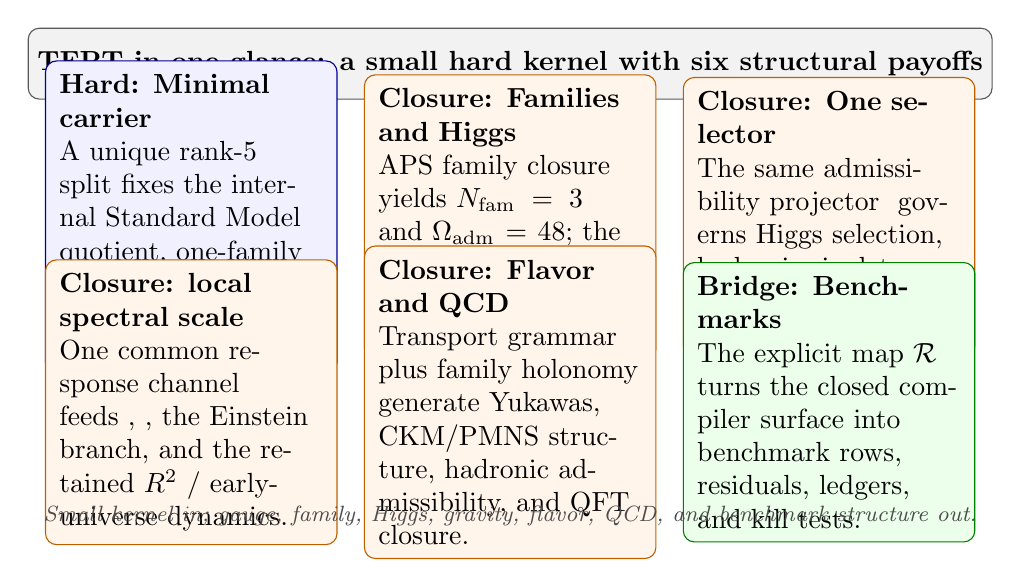
\begin{tikzpicture}[
    headline/.style={draw=black!65, fill=gray!10, rounded corners, minimum width=11.2cm, minimum height=0.9cm, align=center, font=\bfseries},
    hard/.style={draw=blue!60!black, fill=blue!6, rounded corners, text width=3.35cm, minimum height=1.75cm, align=left, inner sep=5pt},
    closure/.style={draw=orange!75!black, fill=orange!8, rounded corners, text width=3.35cm, minimum height=1.75cm, align=left, inner sep=5pt},
    bridge/.style={draw=green!50!black, fill=green!8, rounded corners, text width=3.35cm, minimum height=1.75cm, align=left, inner sep=5pt},
    note/.style={font=\footnotesize\itshape, text=black!70, align=center}
]
\node[headline] (head) at (0,0) {TFPT in one glance: a small hard kernel with six structural payoffs};

\node[hard] (a) at (-4.05,-1.95) {\textbf{Hard: Minimal carrier}\\A unique rank-$5$ split fixes the internal Standard Model quotient, one-family packet, and the hard electromagnetic kernel.};
\node[closure] (b) at (0,-1.95) {\textbf{Closure: Families and Higgs}\\APS family closure yields $N_{\mathrm{fam}}=3$ and $\Omega_{\mathrm{adm}}=48$; the bosonic index selects one light seam-even Higgs doublet.};
\node[closure] (c) at (4.05,-1.95) {\textbf{Closure: One selector}\\The same admissibility projector $\Padm$ governs Higgs selection, hadronic singlets, strong CP, and the vacuum sector.};

\node[closure] (d) at (-4.05,-4.3) {\textbf{Closure: local spectral scale}\\One common response channel feeds $\Mpl$, $\vgeo$, the Einstein branch, and the retained $R^2$ / early-universe dynamics.};
\node[closure] (e) at (0,-4.3) {\textbf{Closure: Flavor and QCD}\\Transport grammar plus family holonomy generate Yukawas, CKM/PMNS structure, hadronic admissibility, and QFT closure.};
\node[bridge] (f) at (4.05,-4.3) {\textbf{Bridge: Benchmarks}\\The explicit map $\mathcal R_{\SM}$ turns the closed compiler surface into benchmark rows, residuals, ledgers, and kill tests.};

\node[note] at (0,-5.75) {Small kernel in; gauge, family, Higgs, gravity, flavor, QCD, and benchmark structure out.};
\end{tikzpicture}
\caption{Headline claims of the present draft. The figure is intentionally simpler than the dependency maps that follow: its job is to put the manuscript's core payoff on one page, while still keeping the hard / closure / benchmark split visible.}
\label{fig:tfpt-headline-claims}
\end{figure}

\begin{tcolorbox}[colback=blue!3, colframe=blue!50!black, breakable,
    title={\textbf{TFPT master equation and selectors}}, fonttitle=\bfseries]
\begin{equation}
\label{eq:tfpt-master}
\begin{aligned}
S_{\mathrm{TFPT}}
=
\operatorname{Tr}f\!\left(\frac{D_{\mathrm{rel}}+A_{\Sigma}^{\mathrm{seed}}}{\chiseed}\right)
-
\operatorname{Tr}f\!\left(\frac{D_{\mathrm{ref}}}{\chiseed}\right)
+\frac{i\pi}{2}\Delta\eta_\Sigma,
\qquad
A_{\Sigma}^{\mathrm{seed}}:=\mathcal B_{\mathrm{rel}}\oplus\nabla_{\chiseed}.
\end{aligned}
\end{equation}
\begin{equation}
\label{eq:tfpt-selectors}
\begin{aligned}
\operatorname*{Stat}_{\alpha,\chiseed,e,\wspin}S_{\mathrm{TFPT}}=0,
\qquad
\Padm:=P_{\Seam,+}P_{\mathrm{sing}}P_\Theta P_{\mathrm{gap}},
\\
\operatorname{Ind}_{APS}(D^+_{\mathrm{rel}}\otimes L_F)=3,
\qquad
\operatorname{Ind}^{\Padm}_{\mathrm{rel}}(\mathcal B^+_{E_2})=1,
\qquad
\operatorname{Ind}^{\Padm}_{\mathrm{rel}}(\mathcal B^+_{E_3})=0.
\end{aligned}
\end{equation}
\end{tcolorbox}

The hard carrier theorems below do not require the full closure stack behind \Cref{eq:tfpt-master,eq:tfpt-selectors}. In the present paper the master equation is the organizing compiler form, the carrier theorems are hard, and the later closure theorems are theorem-level statements relative to the declared admissibility and reflection axioms rather than extra primitive ontology. At this overview level the seed package is written as $A_{\Sigma}^{\mathrm{seed}}$; on the later geometric branch it is reorganized as $A_{\Sigma}^{\mathrm{geo}}$ with $\chiseed\mapsto\chigeo=\Lambda e^\sigma$.

\begin{tcolorbox}[colback=blue!3, colframe=blue!50!black, breakable,
    title={\textbf{Carrier-first compiler chain}}, fonttitle=\bfseries]
\begin{equation}
\label{eq:compiler-chain}
\begin{aligned}
(\widetilde M\to M,\Seam,\inv,\chiseed)
&\Rightarrow
(E_3\oplus E_2,\ G_{\SM}^{\mathrm{glob}},\ S^+)\\
&\Rightarrow
( \Padm,\ N_{\mathrm{fam}}=3,\ F,\ \Oadm=48,\ \Phi)\\
&\Rightarrow
( \Mpl,\ \vgeo,\ Y_f,\ \Hhad,\ \bar\theta )\\
&\Rightarrow
(m_f,\ V_{\mathrm{CKM}},\ U_{\mathrm{PMNS}},\ \Lambda_{\Seam,\mathrm{ren}},\ \Pred).
\end{aligned}
\end{equation}
\end{tcolorbox}

\begin{tcolorbox}[colback=orange!4, colframe=orange!65!black, breakable,
    title={\textbf{Current closed stack and named open theorem obligations}}, fonttitle=\bfseries]
\textbf{Current closed stack:}
\[
\text{primitive datum}
\Longrightarrow
\text{hard carrier kernel}
\Longrightarrow
\text{admissibility closure}
\Longrightarrow
\text{benchmark bridge}.
\]
\textbf{Named open theorem obligations:}
\begin{enumerate}[label=\textbf{O\arabic*:}, leftmargin=1.7em, topsep=3pt, itemsep=2pt]
    \item master closure,
    \item full operator reconstruction,
    \item vacuum-overlap transport closure,
    \item UV Bernstein-cone completion,
    \item cosmology closure,
    \item observation closure.
\end{enumerate}
These six obligations are developed explicitly only later in the paper, but they already control the truth mode of the present draft: current closure is real, while these upgrade theorems remain named future targets rather than silently assumed results.
\end{tcolorbox}

\begin{figure}[t]
\centering
\scriptsize
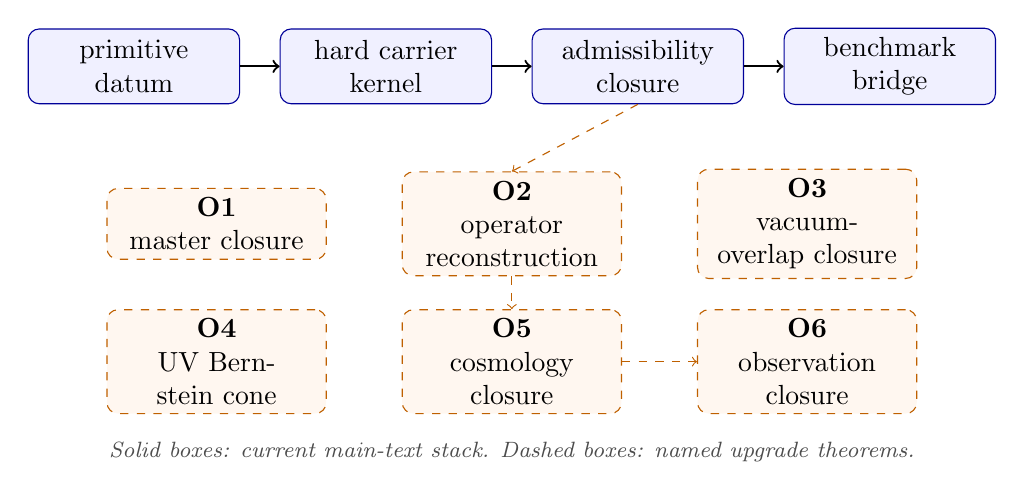
\begin{tikzpicture}[
    closed/.style={draw=blue!60!black, fill=blue!6, rounded corners, text width=2.45cm, minimum height=0.95cm, align=center},
    open/.style={draw=orange!75!black, fill=orange!6, rounded corners, dashed, text width=2.55cm, minimum height=0.9cm, align=center},
    note/.style={font=\footnotesize\itshape, text=black!70, align=center}
]
\node[closed] (p) at (-4.8,0) {primitive\\datum};
\node[closed] (h) at (-1.6,0) {hard carrier\\kernel};
\node[closed] (c) at (1.6,0) {admissibility\\closure};
\node[closed] (b) at (4.8,0) {benchmark\\bridge};
\draw[->, thick] (p) -- (h);
\draw[->, thick] (h) -- (c);
\draw[->, thick] (c) -- (b);

\node[open] (o1) at (-3.75,-2.0) {\textbf{O1}\\master closure};
\node[open] (o2) at (0,-2.0) {\textbf{O2}\\operator reconstruction};
\node[open] (o3) at (3.75,-2.0) {\textbf{O3}\\vacuum-overlap closure};
\node[open] (o4) at (-3.75,-3.75) {\textbf{O4}\\UV Bernstein cone};
\node[open] (o5) at (0,-3.75) {\textbf{O5}\\cosmology closure};
\node[open] (o6) at (3.75,-3.75) {\textbf{O6}\\observation closure};
\draw[->, dashed, orange!75!black] (c.south) -- (o2.north);
\draw[->, dashed, orange!75!black] (o2) -- (o5);
\draw[->, dashed, orange!75!black] (o5) -- (o6);
\node[note] at (0,-4.9) {Solid boxes: current main-text stack. Dashed boxes: named upgrade theorems.};
\end{tikzpicture}
\caption{Status ladder for the present draft. The upper row is the currently closed compiler stack, while the dashed lower row marks the six named upgrade paths carried later in the manuscript.}
\label{fig:status-ladder}
\end{figure}

The remainder of the main text sharpens each arrow of this chain in turn.

\section{Primitive core and hard carrier kernel}

\subsection{Primitive core and conventions}

We use natural units $c=\hbar=1$. Relative operators are formulated in Euclidean signature and compared through a declared Wick-rotation bridge when Lorentzian language is needed. Higgs fields are denoted by $\Phi$, Hamiltonians by $\mathcal H$, and the cosmological Hubble rate by $\Hhub(t)$; this avoids overloading the letter $H$. Newton's constant is always $G_N$, while $G_{\SM}^{\mathrm{glob}}$ is reserved for the global Standard Model gauge quotient. The seam is denoted by $\Seam$, the involution by $\inv$, and word parity by $\varepsilon(w)$.

Here $S\to \widetilde M$ denotes the spinor bundle on the oriented double cover, and by the same symbol we denote its restriction to
\[
X=\widetilde M\setminus\Seam.
\]

When color-center notation is needed later, we use multiplicative notation
\[
z(w)\in\{1,\omega,\omega^2\},
\qquad
\omega=e^{2\pi i/3}.
\]
Thus center neutrality means $z(w)=1$.

\[
\Tcore
:=
\bigl(
\widetilde M\to M,\ \Seam,\ S,\ \Hint,\ \inv,\ D_{\mathrm{rel}},\ f,\ \chiseed
\bigr).
\]
Here \enquote{relative} always means comparison with a declared reference operator or reference-subtracted action. The admissibility predicate $\mathsf{Adm}$ and its operator realization $(\Kadm,\Padm)$ belong to the later closure layer rather than to this primitive bookkeeping package. The technical tables for relative objects, layered closure/benchmark data, and the constants atlas are collected in Appendix~\ref{app:tech} and Appendix~\ref{app:constants}; they are kept out of the early main-text flow so that the carrier kernel appears before the technical bookkeeping apparatus.

\begin{remark}[Assumed datum versus derived structure]
In the present draft the oriented double cover, seam, involution, the relative comparison framework, and the primitive seam response $\chiseed$ are starting data. What is derived from them in hard form is the carrier split, the internal gauge quotient, the one-family packet, the abelian index, and the electromagnetic kernel numerics. The operative selector, family closure, Higgs selection, local spectral-scale closure, transport closure, and Lorentz/vacuum reconstruction belong to the later closure layer and are not folded back into the primitive datum.
\end{remark}

\subsection{Primitive relative spectral dynamics}

The carrier theorem is not intended to float above an unspecified microscopic dynamics. The primitive TFPT datum is therefore stated already at the operator level, before the later closure theorems are invoked.

\begin{definition}[Primitive relative spectral datum]
Let
\[
X:=\widetilde M\setminus \Seam
\]
be the oriented double cover with seam removed. The primitive datum is the genuinely pre-carrier relative spectral package
\[
\Tprim
:=
\bigl(
X,\ S,\ \Hint,\ D_{\mathrm{rel}},\ \inv,\ f,\ \chiseed
\bigr),
\]
with
\[
\mathcal H_{\mathrm{prim}}
:=
L^2(X,S)\otimes \Hint.
\]
Here $\Hint$ is finite dimensional, $\inv$ acts as an involutive grading on $\Hint$, $f$ is a Bernstein spectral test function
\begin{equation}
\label{eq:bernstein-test-function}
f(x)=\int_0^\infty e^{-t x^2}\,d\mu(t),
\qquad
d\mu(t)\ge 0,
\end{equation}
and $\chiseed$ is the primitive seam-even scalar response. The later carrier split $E_3\oplus E_2$, the family space $F$, the gauge adjoint sector, the local spectral scale $\chigeo=\Lambda e^\sigma$, and the operative selector $\Padm$ belong to the hard or closure layers and are not part of $\Tprim$.
\end{definition}

\begin{definition}[Primitive Euclidean action]
The primitive Euclidean action is the relative spectral seed
\[
S_{\mathrm{prim}}[\chiseed]
:=
\tr f\!\left(\frac{D_{\mathrm{rel}}}{\chiseed}\right)
-
\tr f\!\left(\frac{D_{\mathrm{ref}}}{\chiseed}\right)
+\frac{i\pi}{2}\Delta\eta_\Sigma.
\]
Gauge fixing, ghosts, carrier-compatible bosonic fluctuations, and the admissibly compressed net
\[
\mathfrak A_{\mathrm{adm}}(\mathcal O):=
\Padm\,\mathfrak A(\mathcal O)\,\Padm.
\]
are introduced only after the hard carrier theorem and the later admissibility closure package are in place.
\end{definition}

\begin{assumption}[Bernstein positivity input]
\label{ass:bernstein-positivity}
On the admissible bosonic sector used later in the closure layer, the relevant comparison operator admits a Bernstein heat-kernel representation with a positivity-preserving semigroup on the seam-even branch, and this sector is reflection-stable.
\end{assumption}

\begin{proof}[Proof sketch]
For every $t>0$, the operator $e^{-tD_{\mathrm{rel}}^2/\chiseed^2}$ is the heat semigroup of a Dirac-square-type kernel on the primitive bosonic sector. Positivity of the heat kernel is preserved under positive superposition with $d\mu(t)\ge0$, so the Bernstein representation keeps the semigroup positivity and ordering structure intact. Admissibility compression and the fermionic CAR reconstruction are only added later, after the hard carrier and closure packages have been identified.
\end{proof}

\begin{theorem}[Well-posed primitive dynamics]
Assume $X$ is compact up to the elliptic boundary domain $\APSdom$, the coefficients of $D_{\mathrm{rel}}$ are smooth, and the Bernstein measure in \Cref{eq:bernstein-test-function} has finite moments of every order. Then:
\begin{enumerate}[label=(\alph*), leftmargin=1.5em, topsep=3pt, itemsep=2pt]
    \item $D_{\mathrm{rel}}$ is essentially self-adjoint on the $\APSdom$ domain;
    \item $D_{\mathrm{rel}}$ has compact resolvent on the finite-cutoff Euclidean branch;
    \item the spectral action trace is finite for every finite cutoff;
    \item and the finite-cutoff relative Euclidean seed defines a well-posed primitive dynamics before carrier and admissibility closure are imposed.
\end{enumerate}
\end{theorem}

\begin{proof}[Proof sketch]
Dirac-type operators with $\APSdom$ boundary data are Fredholm and essentially self-adjoint on the corresponding Sobolev domain. Compactness of the resolvent follows on compact $X$ with $\APSdom$ boundary, while the Bernstein representation with finite moments makes the spectral trace finite at every finite cutoff. This yields a well-defined primitive relative spectral seed before any later carrier-compatible fluctuation package is turned on.
\end{proof}

\begin{remark}[Two APS layers]
The manuscript uses APS language in two distinct roles. The primitive layer needs only the elliptic domain choice $\APSdom$ for self-adjointness and Fredholm control of $D_{\mathrm{rel}}$. The later family-closure layer needs additional pairing data $\APSfam$ on $\Seam$ to formulate the orbifold--APS family theorem and its compatibility with the admissibility complex. Keeping $\APSdom$ and $\APSfam$ separate prevents the family theorem from being mistaken for part of the primitive input package.
\end{remark}

\begin{figure}[t]
\centering
\scriptsize
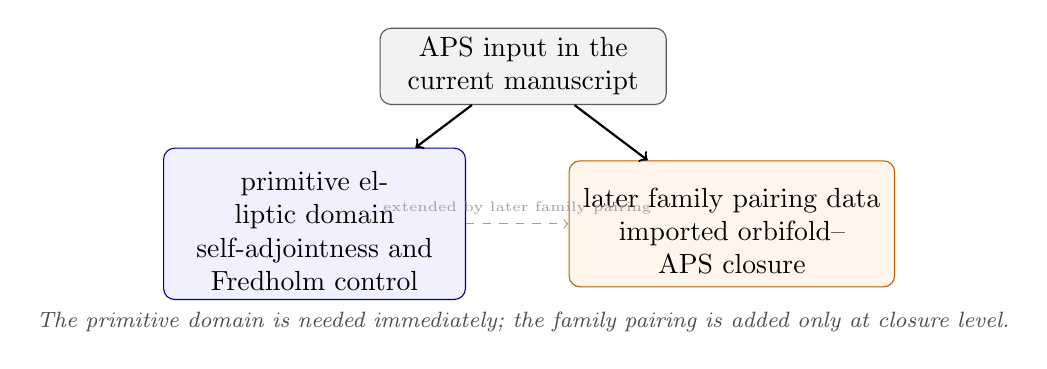
\begin{tikzpicture}[
    root/.style={draw=black!65, fill=gray!10, rounded corners, text width=3.4cm, minimum height=0.9cm, align=center},
    dom/.style={draw=blue!60!black, fill=blue!6, rounded corners, text width=3.6cm, minimum height=1.6cm, align=center},
    fam/.style={draw=orange!75!black, fill=orange!8, rounded corners, text width=3.9cm, minimum height=1.6cm, align=center},
    note/.style={font=\footnotesize\itshape, text=black!70, align=center}
]
\node[root] (aps) at (0,0) {APS input in the current manuscript};
\node[dom] (dom) at (-2.65,-2.0) {\textbf{$\APSdom$}\\primitive elliptic domain\\self-adjointness and Fredholm control};
\node[fam] (fam) at (2.65,-2.0) {\textbf{$\APSfam$}\\later family pairing data\\imported orbifold--APS closure};
\draw[->, thick] (aps) -- (dom);
\draw[->, thick] (aps) -- (fam);
\draw[->, dashed, gray!75] (dom.east) -- node[above, sloped] {\tiny extended by later family pairing} (fam.west);
\node[note] at (0,-3.25) {The primitive domain is needed immediately; the family pairing is added only at closure level.};
\end{tikzpicture}
\caption{APS split in the present draft. $\APSdom$ handles primitive elliptic well-posedness, while $\APSfam$ is the later family-pairing layer needed for the imported orbifold--APS family theorem.}
\label{fig:aps-split}
\end{figure}

\begin{corollary}[Carrier-compatible Lorentzian dynamics after closure]
Once the later carrier-compatible fluctuation package and the admissibility closure hypotheses of \Cref{sec:closure-theorems} are imposed, the resulting admissible Euclidean theory reconstructs a self-adjoint Lorentzian Hamiltonian $H_{\mathrm{adm}}$ and a one-parameter automorphism group
\[
\alpha_t(O)=e^{itH_{\mathrm{adm}}}Oe^{-itH_{\mathrm{adm}}}.
\]
\end{corollary}

